\documentclass[12pt, oneside]{article}   	% use "amsart" instead of "article" for AMSLaTeX format
\usepackage{textcomp}
\usepackage{geometry}                		% See geometry.pdf to learn the layout options. There are lots.
\geometry{letterpaper}                   		% ... or a4paper or a5paper or ... 
%\geometry{landscape}                		% Activate for rotated page geometry
%\usepackage[parfill]{parskip}    		% Activate to begin paragraphs with an empty line rather than an indent
\usepackage{graphicx}				% Use pdf, png, jpg, or eps§ with pdflatex; use eps in DVI mode
\usepackage{caption}
\usepackage{subcaption}								% TeX will automatically convert eps --> pdf in pdflatex		
\usepackage{color}
\usepackage{amssymb}
\usepackage{amsthm}
\usepackage{url}
\newtheorem{theorem}{Theorem}
\newtheorem{definition}{Definition}
\usepackage{natbib}
\usepackage{xcolor}
% removed hyperref because of arXiv complaining
\usepackage{authblk}
\usepackage{float}
\usepackage{rotating}
\usepackage{adjustbox}
\usepackage[font=small,labelfont=bf]{caption}
%\usepackage{changes}
\usepackage{changes}
\definechangesauthor[name={George Chacko}, color=blue]{gc}

\usepackage{authblk}
\title{Finding Well-Connected Communities in Real-World Networks}
\author[1]{Minhyuk Park\thanks{author order to be determined later}}
\author[1]{Yasamin Tabatabaee\thanks{author order to be determined later}}
\author[1]{Baqiao Liu\thanks{author order to be determined later}}
\author[1]{Placeholder1\thanks{author order to be determined later}}
\author[1]{Placeholder2\thanks{author order to be determined later}}
\author[1]{Placeholder3\thanks{author order to be determined later}}
\author[2]{Dmitriy Korobskiy}
\author[1,3]{George Chacko\thanks{chackoge@illinois.edu}}
\author[1]{Tandy Warnow\thanks{warnow@illinois.edu}}
\affil[1]{Department of Computer Science, University of Illinois Urbana-Champaign, Urbana, IL 61801}
\affil[2]{NTT DATA, McLean, VA 22102}
\affil[3]{Office of Research, Grainger College of Engineering, University of Illinois Urbana-Champaign, Urbana, IL 61801}

% \setlength{\parindent}{0pt}
%SetFonts

% ORCID IDs

% Baqiao Liu: 0000-0002-4210-8269
% Tandy Warnow: 0000-0001-7717-3514
% George Chacko: 0000-0002-2127-1892

\begin{document}
\maketitle
	
\abstract{Community detection in real-world networks is typically addressed through the use of graph clustering methods that partition the nodes of a 
network into disjoint subsets. While  the definition of community varies across methods, it is generally accepted that a elements of a community 
should be ``well-connected". 
Here, we explore features of clusters generated by the Leiden algorithm  and the Iterative K-core clustering algorithm. We evaluate 
clusters that are produced  by these two approaches for their susceptibility to become disconnected by the deletion of a small number of edges, and find that both methods produce some 
clusters that are poorly connected  when applied to real-world networks.  
We present a new pipeline to enable 
well-connected output clusters, which allows a user to specify the criterion for a valid  community in terms of the minimum edge cut size as a function of the cluster size. We describe the 
use of this pipeline on real world networks and  synthetic LFR networks.
The differences we observe between real world and synthetic LFR networks are striking: while many clusters produced on real-world networks are poorly connected, clusters computed on LFR networks  are nearly always well-connected, and 
most of the LFR network is thus covered by well-connected clusters.
Since a basic assumption of the LFR network generation process is that every vertex  is in a community, this  study suggests the possibility that community structure is not globally found within real-world networks, and that clusters produced by standard methods  should be further evaluated. 
}
	
\clearpage
	
\section{Introduction} 

The problem of finding communities in complex networks can be posed as a {\em graph partitioning} problem, where the input is a network (a graph with vertices and edges) and the
objective is a partitioning of the vertices into disjoint subsets, so that each of the subsets represents a community \citep{Girvan_2002,Newman_2004}. Community 
detection in  large networks has broad applications that include, in scientometrics, the detection of research areas, and author communities \citep{Waltman_2012,Li2014,Fiallos2017,Traag_2019,Chandrasekharan_2020,Wedell2022}.

While variations of the disjoint partition theme arise from different scientific interests \citep{Coscia2011,Schaub2017}, it is a  common approach to community detection that has been used in many 
studies \citep{Fortunato2022,Fortunato2010}.
Moreover, a common feature of the different formulations of community detection is that  the elements of a community are more connected to each other than to those outside the community. 
In other words, a community should be {\em well-connected}.
Using graph-theoretic terminology, a cluster is said to be well-connected if it does not have a small 
edge cut, which means that there should not be a small set of edges whose deletion disconnects the cluster; see discussion in \cite{Traag_2019}. 

While the concept of being well-connected depends on the size of the edge cut, the definition of what is ``too small" can be formulated in two
natural ways.
The first way
requires that an edge cut  $E_0$ be above some value derived from the number $n$ of 
vertices in the cluster $C$ such as $$||E_0|| \geq \log_{10}(||C||),$$    where $||.||$ denotes the number of elements in the given set.
Note that every edge in  a tree cluster is a cut edge, and so is  a compelling example of a poorly connected cluster. 
Note also that this is a relatively weak bound for large clusters (i.e., when   $n$ is large), but does provide some constraints on small clusters. 

The second approach, which is used in providing guarantees for the widely used Leiden algorithm \citep{Traag_2019}, evaluates the size of an edge cut by the split  of the cluster into two parts produces 
when the edge cut is removed from a cluster, and requires that the edge cut size be at least a fraction of the number of possible edges between the two  parts.
As proven, Equation D1 in the supplementary information in \cite{Traag_2019}, given any optimal CPM clustering of a network using resolution parameter $\gamma$, if an edge cut $E_0$
separates a cluster into two sets $A$ and $B$ then $$||E_0|| \geq \gamma ||A|| \times ||B||$$
This is a strong guarantee when the cluster is large,  but as it depends on the user-specified value for $\gamma$, it may have no guarantee  beyond being connected for small clusters.
Thus, the two approaches provide guarantees about clusters being well-connected for different size clusters, with the first approach a stronger guarantee for small to moderate-sized clusters, and the second approach providing a stronger guarantee on the larger clusters.

Given the importance of communities being well-connected, we performed a study to evaluate the question of whether clusters produced by two different clustering methods
were consistently found to be well-connected, using the first criterion we pose, so that for every cluster, the minimum edge-cut size must be greater than $\log_{10}n$, where $n$ is the number of vertices in the cluster. 
We used a collection of real-world networks in our study, including some citation graphs.
This evaluation showed that both Leiden and IKC clusterings produced clusters that failed to be well-connected according to this criterion.
The results depended on the resolution parameter selected for Leiden,  with a higher incidence of failure for small values for the resolution parameter.

We then designed a pipeline to work with both Leiden and IKC that would ensure that all output clusters satisfy two constraints for being valid communities: (1) they are well-connected according to our criterion, and (2) each cluster meets a minimum user-specified size requirement. The pipeline takes the clustering as input, and first finds and removes all clusters that are either trees or are too small.  It then checks each remaining cluster for being well-connected; if a cluster fails this check so that it has a small edge cut, the minimum edge cut is deleted from the cluster, thus producing a set of subsets.  Each of these subsets are then re-clustered using the selected clustering method (IKC or Leiden), and the process recurses on the resultant set of clusters.

Our study using this pipeline on a collection of real-world networks shows some surprising results. First, we find that the final clustering produced using Leiden, across a range of resolution values, 
covered only a portion of the input network, with a  fraction that ranged from x\% to y\% of the vertices. \textcolor{blue}{pending rewrite}.

\textcolor{blue}{TO do:
\begin{itemize}
\item Report the fraction of input clusters that fail our test as a function of the cluster size.
We expect this to be a large fraction for small clusters but it may continue into the larger clusters.
Will be good to note.
\item Look at how much of the network is in the *union* of the output (post-pipeline) clusterings, across the Leiden resolution parameter values.
\item Compute the overlap between clusterings both pre-pipeline and post-pipeline
\item  Maybe? Evaluate accuracy of Leiden clusterings on LFR networks 
\end{itemize}
}

\section{Materials and Methods}

\subsection{Methods} 
\emph{Pipeline Design} A modular pipeline was developed that (i) generated a clustering from an input network using one of three methods,  (ii) filtered the resultant clusters to remove small clusters and trees,  (iii) applied \emph{Connectivity Modifier} (CM), a recursive  method that modifies the clustering to ensure that all output clusters are well-connected, and (iv) remove all clusters below size $B$ (where $B=11$ by default).

The three clustering methods we enabled are Leiden for CPM with resolution parameter $r$, Leiden for modularity optimization, and Iterative k-core (with parameter $k$ set by default to $10$).
For  a cluster $C$ to be considered``well-connected", we require that the size of the minimum edge cut for $C$ be greater than $\log_{10}(||C||)$ (where $||C||$ denotes the number of vertices in $C$), but this
is a parameter that can be modified by the user.  
These steps are described below in greater detail. 

\vspace{5 mm}
\textbf{[Insert flow chart of workflow/pipeline]}

\subsubsection{Clustering} We used either the Python implementation of the Leiden algorithm [add Github reference] or the Iterative K-core Clustering (IKC) algorithm [add Github reference].

\subsubsection{Filters} Three different approaches were used to take as input a clustering and a minimum size requirement $B$, and then filter out trees and any cluster of size less than $B$:  (i) Belinda, a Python package [insert Github reference to https://github.com/illinois-or-research-analytics/belinda] for clustering analysis, (ii) a Python script that uses the Networkit library \citep{Staudt2016} to compute edge and node counts for each cluster, and (iii) an R script that computed edge and node counts for clusters (see Supplementary Materials). 
All three returned the same output on test cases. 

\subsubsection{Connectivity Modifier} To recursively compute and apply minimum cuts to individual clusters, we used the Connectivity Modifier (CM) code at [insert Github reference to Connectivity Modifier], which uses Viecut \citep{Henzinger2018,Henzinger2019} as a dependency, and takes as input a clustering from either the Leiden algorithm or IKC, and returns a set of clusters that is guaranteed to be
well-connected. 
We filtered the input clustering as above before passing it as input to Connectivity Modifier. [insert references https://pypi.org/project/connectivity-modifier/].

Here we describe the CM code when passed an input  Leiden clustering $\mathcal{C}$  with resolution parameter $r$; modifying this description to work with 
Leiden for modularity or IKC is then straightforward.
CM used with Leiden and parameter $r$ has the following structure.


First, the set $Bin$ is initialized to the empty set  ($\emptyset$).
CM  then orders the clusters in the input clustering into a queue,  marks them as ``clustered", and processes each cluster in the queue in turn.
Given a cluster $C$ in the queue, if it is marked as ``clustered" then CM uses VieCut to find a small cut in $C$;  if the cut is at most $\log_{10}(||C||)$ (where $||C||$ denotes the number of 
vertices in the cluster), then it removes the cut from the network, splitting the cluster $C$ into two  subsets $A$ and $B$.
Both $A$ and $B$ are then added into  queue for subsequent processing, and marked as ``new". 
If the cut size for $C$ was above $\log_{10}(||C||)$, then $C$ is added to $Bin$.
Given a cluster $C$ in the queue that is marked as ``new", it uses Leiden with resolution parameter $r$ on the cluster, thus reclustering $C$
and potentially breaking it up into many subsets; each of these subsets is then added to the queue and marked as ``clustered".
When the queue is empty, the clusters in $Bin$ are returned as the output.

Note that the structure of the CM algorithm ensures that every cluster $C$ in the output is well-connected, since it is 
placed in $Bin$ only if the cut found by VieCut is above $\log_{10}(||C||)$.
However, the CM code as described does not enforce a size constraint.

\textcolor{blue}{For Minhyuk: provide latex for pseudo-code that we can put in the supplement. Make sure it reflects how the algorithm is implemented. On the other hand, and very importantly, the README for the github site says the CM code is a DFS, so this uses a stack and not a queue.  If this is in fact how the algorithm is implemented, then what I wrote is wrong. This needs clarification.}

\subsection{The CM pipeline}
The entire CM pipeline operates in three stages, taking as input (a) the
network $N$,  (b) a clustering method (either Leiden for CPM, Leiden for modularity, or Iterative k-core) with the required
parameter values (e.g., resolution value for Leiden with CPM and value for $k$ for IKC),
(c)  the initial clustering $\mathcal{C}$ of $N$ using the selected clustering method, 
(d) the required minimum size $B$ for the output clusters (default $B=11$)
and (e) the bound on the minimum cut size as a function of the number of vertices in the cluster $C$
(default $\log_{10}(||C||))$).

\begin{itemize}
\item Stage 1: We perform the filtering, which removes all clusters that are trees or that are below size $B$ from $\mathcal{C}$
\item Stage 2: We run CM on the remaining clusters, returning a set of clusters that are all well-connected
\item Stage 3: We remove all clusters that are below size $B$ or that are trees
\end{itemize}




%\begin{itemize} %(2)
%\item $Bin = \mathcal{C}$
%\item While $Bin \neq \emptyset, DO$
%\begin{itemize}  %(3)
%\item 
%For $C \in Bin$ DO
%\begin{itemize}
%\item If VieCut finds a cut $E$ for cluster $C$ of size at most $\log_{10}(||C||)$, then
%\begin{itemize} %(4)
%\item 
%(a)  delete $E$ from the network, thus splitting the cluster $C$ into two components $A$ and $B$, 
%(b)  Add $A$ and $B$ to $Bin'$, and (c) Delete $C$ from $Bin$
%\end{itemize} %4
%\end{itemize} %3
%\item 
%If $Bin' \neq \emptyset$ then for each cluster $C \in Bin'$:
%\begin{itemize} %5
%\item Remove $C$ from $Bin'$
%\item Apply Leiden with parameter $r$ to recluster  $C \in Bin'$, and add the resulting 
%clusters to $Bin'$
%\end{itemize} %5
%\end{itemize} %2
%\end{itemize}



\subsection{Data} Several networks were used for testing and analysis and were selected to provide a range of sizes and edge density. In all cases, below the counts of nodes and edges are reported after removing duplicate records, 
self-citations, and parallel edges from the source data. 


\paragraph{Curated Exosome Network (CEN)}
The CEN is centered around the exosome research literature. and it consists of 13,989,436 nodes and 92,051,051 edges and its construction has previously been previously described in \cite{Jakatdar_2022}.  

\paragraph{Open Citations}
A custom-implemented ETL process was designed to process the publicly available OpenCitations dataset \citep{Peroni2020} and load it into a PostgreSQL table. Citation data (CSV) was downloaded in Aug 2022. A custom ETL script, written in Bash and SQL, was used to find and pipe uncompressed CSV files, in 20 parallel jobs using the GNU Parallel command-line utility, to a custom function which loaded individual CSV files into a staging view. DOIs were also checked for case differences to remove duplicates.  The resultant network contained 75,025,194 nodes and 1,363,605,603 edges.  
The Open Citations dataset was large enough that evaluating every cluster was not feasible. Thus, samples were used for analysis by connectivity modifier. Briefly, non-tree samples of size at least 11 were divided into deciles based on cluster sizes and 5\% of each decile was randomly sampled. Where decile values were similar, multiple samples were taken. For example, when the Open Citations data was clustered with the Leiden algorithm at resolution value of 0.5, the first, second, and third deciles were equal to 11. Thus three 5\% samples were taken from the class $x=11$ with replacement and de-duplicated after collection. 

% latex table generated in R 4.1.3 by xtable 1.8-4 package
% Sun Jan 22 19:56:56 2023
\begin{table}[ht]
\centering
\resizebox{.5\textwidth}{!}{
\begin{tabular}{rrrrrll}
  \hline
 & clus\_count & min & med & max & type & gp \\ 
  \hline
1 & 20648920 &   2 &   2 &  10 & size 2-10 & leiden.5 \\ 
  2 & 297038 &  11 &  13 & 183 & size $>$10 & leiden.5 \\ 
  3 & 297038 &  11 &  13 & 183 & non\_tree & leiden.5 \\ 
  4 & 10349 &  11 &  13 &  85 & pre-cm & leiden.5 \\ 
  5 & 10349 &  11 &  13 &  85 & post-cm & leiden.5 \\ 
  \hline
  6 & 7324830 &   2 &   5 &  10 & size 2-10 & leiden.1 \\ 
  7 & 1313856 &  11 &  17 & 882 & size $>$10 & leiden.1 \\ 
  8 & 1299838 &  11 &  17 & 882 & non\_tree & leiden.1 \\ 
  9 & 14016 &  11 &  11 &  11 & star & leiden.1 \\ 
  10 &   2 &  11 &  11 &  11 & tree & leiden.1 \\ 
  11 & 45252 &  11 &  15 & 306 & pre-cm & leiden.1 \\ 
  12 & 39954 &  11 &  16 & 306 & post-cm & leiden.1 \\ 
  \hline
  13 & 772769 &   2 &   2 &  10 &  size 2-10 & leiden.01 \\ 
  14 & 1361168 &  11 &  19 & 3530 & size $>$10 & leiden.01 \\ 
  15 & 1034558 &  11 &  24 & 3530 & non\_tree & leiden.01 \\ 
  16 & 8669 &  11 &  18 & 101 & star & leiden.01 \\ 
  17 & 317941 &  11 &  15 &  58 & tree & leiden.01 \\ 
  18 & 36171 &  11 &  21 & 1561 & pre-cm & leiden.01 \\ 
  19 & 29793 &  11 &  16 & 1561 & post-cm & leiden.01 \\ 
  \hline
  20 & 606966 &   2 &   2 &  10 & size 2-10 & leiden.001 \\ 
  21 & 232288 &  11 &  64 & 23470 & size $>$10  & leiden.001 \\ 
  22 & 208543 &  11 &  73 & 23470 & non\_tree & leiden.001 \\ 
  23 & 1476 &  11 &  15 & 1001 & star & leiden.001 \\ 
  24 & 22269 &  11 &  43 & 500 & tree & leiden.001 \\ 
  25 & 7299 &  11 &  63 & 12707 & pre-cm & leiden.001 \\ 
  26 & 11766 &  11 &  43 & 12707 & post-cm & leiden.001 \\ 
  \hline
  27 & 522696 &   2 &   2 &  10 & size 2-10 & leiden.0001 \\ 
  28 & 39069 &  11 & 177 & 176557 & size $>$10 & leiden.0001 \\ 
  29 & 34031 &  11 & 206 & 176557 & non\_tree & leiden.0001 \\ 
  30 & 3525 &  11 &  14 & 267 & tree & leiden.0001 \\ 
  31 & 1513 &  11 &  14 & 251 & star & leiden.0001 \\ 
  32 & 1192 &  11 & 172 & 53195 & pre-cm & leiden.0001 \\ 
  33 & 1971 &  11 & 118 & 51053 & post-cm & leiden.0001 \\ 
   \hline
\end{tabular}}
\caption{test- data being revised to use larger samples}
\end{table}


\paragraph{SNAP benchmarks}
In addition, four more real world networks from the Stanford Network Analysis Project (SNAP) collection \citep{leskovec2016snap} were downloaded in Dec 2022:
\begin{itemize}
\item  \emph{cit\_patents} (3,774,768 nodes, 16,518,947 edges), \
\item emph{cit\_hepph} (34,546 nodes, 420,877 edges),
\item  \emph{wiki\_topcats} (1,791,489 nodes, 25,444,207 edges), and
\item  \emph{orkut} (3,072,441 nodes, 117,185,083 edges). 
\end{itemize}




\paragraph{LFR (random) networks}
As a comparison group, synthetic networks were generated using the LFR `benchmark' methodology \citep{Lancichinetti2008}. [Ask Yasamin to write this section up].

\textcolor{blue}{
To do (for Yasamin):}

\begin{itemize}
\item For  the CEN and  for the Open Citations networks, produce one LFR network  that has a mixing parameter and other
parameters set so as to produce something that resembles the given Leiden clustering of the given real-world network. (However, keep the LFR network
on the moderate size, so at most 3,000,000 vertices.) 
\textcolor{blue}{This requires that George specify the Leiden clustering for these two networks.}
\item 
For each LFR network: 
\begin{itemize}
\item Report empirical statistics of the network
\item Report empirical statistics of the true clustering 
\item 
Recluster using Leiden (same resolution value) and then run the CM pipeline.
Record all the usual statistics
\item Run CM on the true clustering.
Report all the usual statistics
\end{itemize}
\end{itemize}

\noindent
The usual statistics are things like:
\begin{itemize}
\item Statistics before running the CM pipeline, including distribution of cluster sizes, node and edge coverage 
\item Statistics at each stage of the CM pipeline (percentage of clusters that are deleted due to being trees,
then deleted due to being too small, then the percentage of remaining clusters  that have small edge cuts).
But at the end of the pipeline we also remove small clusters.  
Also show total node and edge coverage at the end of each stage of the CM pipeline. 
\item 
In essence we want to know which clusters in the input survive the entire process, which ones are modified. 
We'll want their sizes as well, so we can say things like ``20\% of the input clusters above size 100 have small edge cuts" and
``10\% of the input clusters above size 50 are trees".
\end{itemize}

\section{Experimental study}
We plan five experiments:

\begin{itemize}
\item Experiment 1: Analyses  for the CEN using Leiden+CM
\item Experiment 2: Analyses of Open Citations using Leiden+CM
\item Experiment 3: Analyses of LFR using Leiden+CM
\item Experiment 4: Analyses of SNAP benchmarks using Leiden+CM
\item Experiment 5: Focused analysis of convergence of Leiden+CM clusters in CEN, looking at IKC as well
\end{itemize}


\section{Results and Discussion}

\emph{Overview editorial for consideration by authors. We need to agree on a vision to integrate the Leiden and IKC results into an overarching hypothesis-driven framework. What is it that we're looking for or trying to say? To me, the answer is in an improved understanding of how the the properties of networks affect clustering and the converse- how clustering methods influence interpretation of the networks that are fed to them. Are we asking too much of ourselves? Should the IKC effort be in its own paper? My sense is that IKC is a valuable comparison method because of the way in which it is so different from Leiden and perhaps less valuable because it's so different from Leiden.}

\textcolor{blue}{\emph{Assuming that we want to have `our very best figure' early, if not first, what should it be?}} I think it should be the CEN tree figure, which would justify exploring other networks.  Does this distract from the focus on connectivity modifier?

\begin{figure}[H]
\centering
%:

%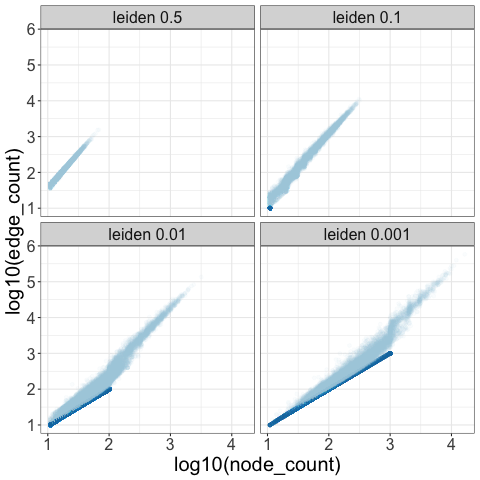
\includegraphics[width=0.7\linewidth]{cen_quad_fig1.png}
\caption{The Curated Exosome Network (CEN) consists of 13,989,436 nodes with average degree of 13.16. The CEN was clustered at four resolution values (0.5, 0.1, 0.01, 0.001) using the Leiden algorithm with Constant Potts Model as quality function. The figure shows the count of edges in each cluster of size $>$  10 plotted against the count of nodes in each cluster (cluster size). Tree clusters are colored green.  resolution values is decreased, node coverage defined here as the fraction of nodes in the network that are found in clusters of size $>$  10, increases. The number of such clusters does not, however, monotonically increase (Table 1). As the resolution value is decreased, the number of tree clusters (dark blue) increases. At a resolution value of 0.01, 84.45\% of network nodes are found in 65,771 clusters of size $>$ 10. Of these 65,771 clusters, 35\% are trees.}
\end{figure}

% latex table generated in R 4.2.2 by xtable 1.8-4 package
% Sun Jan 15 17:20:47 2023
\begin{table}[ht]
\centering
\begin{tabular}{llrrrr}
  \hline
 Clustering  & Resolution &  \# clusters & node coverage & edge coverage \\ 
  \hline
leiden &  0.5 & 8503 & 0.97 & 0.93 \\ 
leiden&  0.1 & 273420 & 23.98 & 7.35 \\ 
leiden & 0.01 & 275641 & 76.52 & 24.39 \\   
leiden& 0.001 & 65771 & 84.45 & 39.01 \\ 
   \hline
\end{tabular}
\caption{Properties of Leiden clusters on the CEN. We show empirical statistics  (cluster count, percentage of vertices in non-singleton clusters (or is this clusters of size at least 11?), and percentage of edges in these clusters) for for Leiden clusterings on the Curated Exosome Network (CEN), using the Constant Potts Model (CPM) as quality function and with different resolution values.
\label{table1}
 }
\end{table} 

% latex table generated in R 4.2.2 by xtable 1.8-4 package
% Sun Jan 15 17:37:03 2023
\begin{table}[ht]
\centering
\begin{tabular}{lrllrrr}
  \hline
 Clustering & Resolution & type & min & med & max \\ 
  \hline
leiden & 0.5 & non\_tree &  11 & 14 &  68 \\ 
leiden & 0.5 & tree &  NA & NA &  NA \\ 
leiden & 0.1 & tree &  11 & 11 &  11 \\ 
leiden  & 0.1 & non\_tree &  11 & 20 & 319 \\ 
leiden  & 0.01 & tree &  11 & 27 & 101 \\ 
leiden & 0.01 & non\_tree &  11 & 34 & 3186 \\ 
leiden & 0.001 & tree &  11 & 65 & 1001 \\ 
leiden & 0.001 & non\_tree &  12 & 112 & 16481 \\ 

   \hline
\end{tabular}
\caption{Cluster sizes for Leiden clusters on the CEN. We show empirical statistics (minimum, median, and maximum) of Leiden clusters, after removing all clusters of size at most 10,  for trees and non-trees, for of the Curated Exosome Network (CEN),  using the Constant Potts Model (CPM) as quality function and with different resolution values.  }
\end{table}



	
\begin{figure}[H]
\centering
\begin{subfigure}[t]{0.48\textwidth}
\centering
%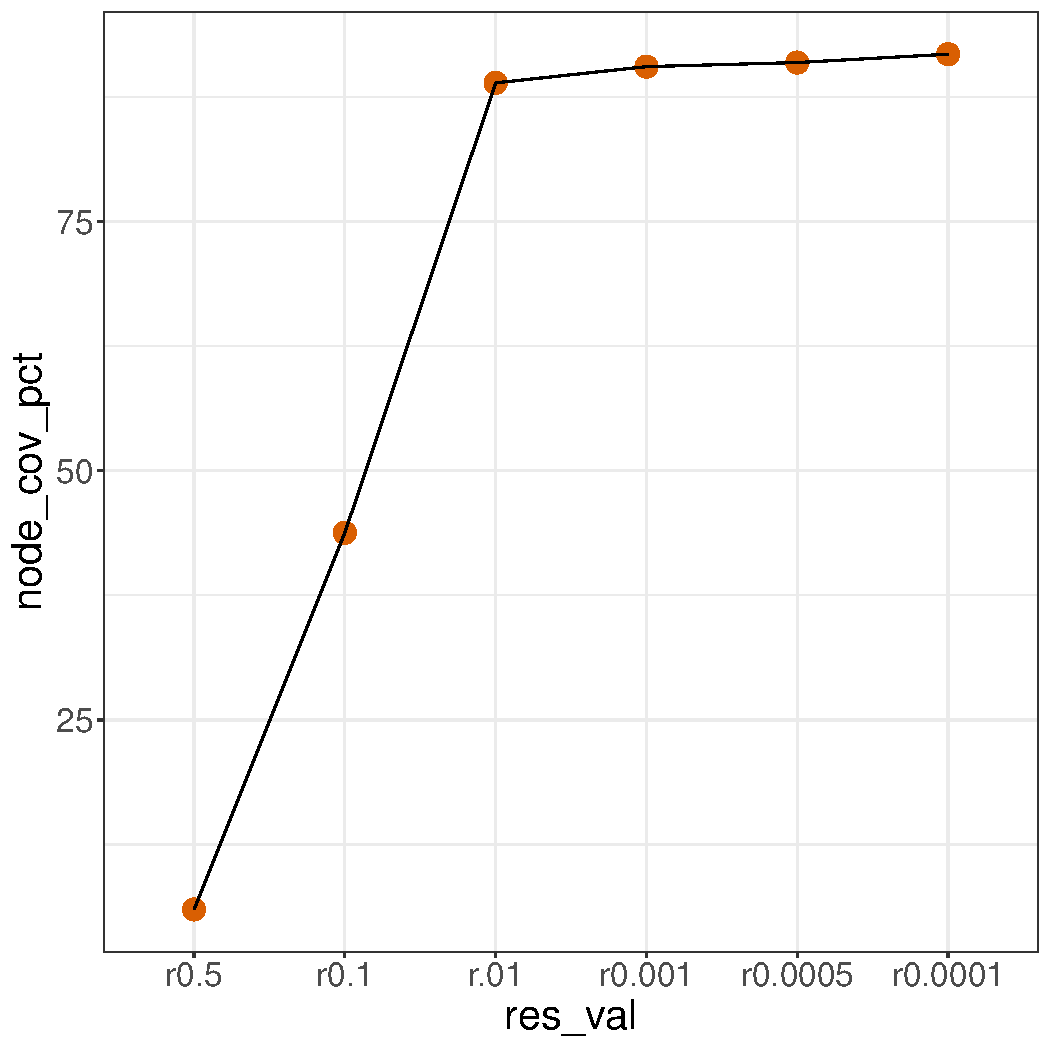
\includegraphics[width=\linewidth]{node_cov.pdf}
\end{subfigure}
\hfill
\begin{subfigure}[t]{0.48\textwidth}
\centering
%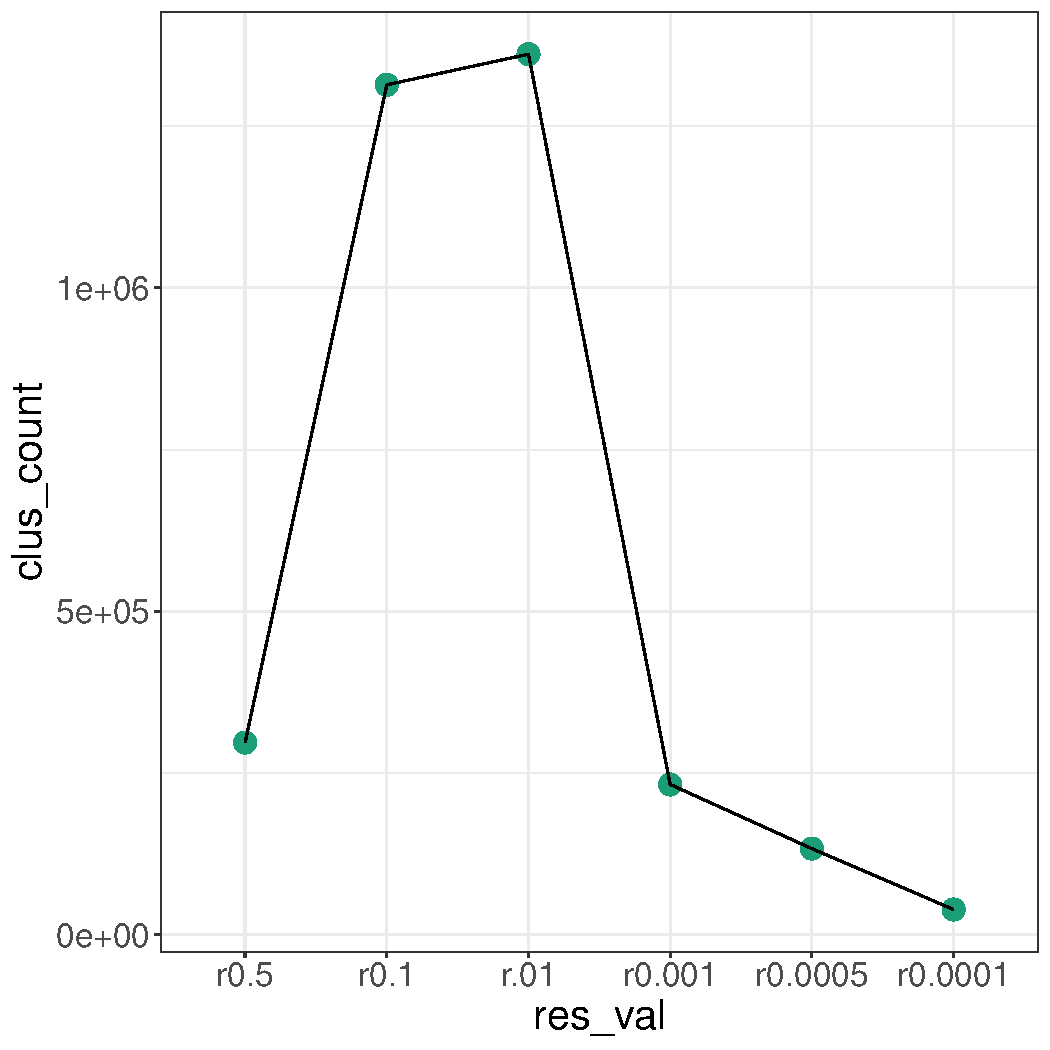
\includegraphics[width=\linewidth]{clus_count.pdf} 
\end{subfigure}
\captionsetup{width=0.9\textwidth}
\caption{Draft Comments: As res\_val decreases, node coverage increases although the number of N$>$10 clusters first goes up then falls. Thus cluster size must be increasing. See Table 1 Maybe this should first be done with CEN clusters?
}
\label{fig:overlapping}
\end{figure}

% latex table generated in R 4.2.2 by xtable 1.8-4 package
% Fri Jan 13 18:03:02 2023
\begin{table}[ht]
\centering
\begin{tabular}{lrrrrrr}
  \hline
 clustering & res\_value & clus\_count & node\_cov & min & med & max \\ 
  \hline
Leiden & 0.5 & 297038 & 5.98 &  11 & 13.00 & 183 \\ 
Leiden & 0.1 & 1313856 & 43.78 &  11 & 17.00 & 882 \\ 
Leiden & 0.01 & 1361168 & 88.93 &  11 & 19.00 & 3530 \\ 
Leiden & 0.01 & 232288 & 90.56 &  11 & 64.00 & 23470 \\ 
Leiden & 0.0005 & 133147 & 90.97 &  11 & 90.00 & 39049 \\  
Leiden & 0.0001 & 39069 & 91.81 &  11 & 177.00 & 176557 \\ 
   \hline
\end{tabular}
\caption{Clustering the Open Citations Network. The open citations network (Materials and Methods) consisting of 75,025,194 nodes and 1,363,605,603 edges was clustered with the Leiden algorithm, using the Constant Potts Model (CPM) as quality function, and using various resolution values (column 1). Node coverage is expressed as the the percent of nodes in these clusters of size $>$ 10 relative to the total number of nodes in the network. Minimum, median, and max cluster sizes are shown in the last three columns.  }
\end{table}


		
\section{Conclusions}
	
\section*{Competing Interests} \vspace{3mm} The authors have no competing interests. 
	
\section*{Funding Information} 
	
\section*{Data Availability} 
	
\section*{Acknowledgments} 

\bibliographystyle{apalike}
\bibliography{cmv1}
\end{document}


